%\documentclass[../main.tex]{subfiles}
%\begin{document}
Process mining is a relatively new discipline that has emerged from the need to bridge data mining and business process management. The objective of process mining is to support the analysis of business process, provide valuable insights on processes and further improve the business execution. According to \cite{van2011process}, techniques of process mining are divided into three categories: process discovery, conformance checking and process enhancement. Process discovery techniques focus on deriving process models from event logs of the information system, allowing the vision into the real business process. Conformance checking analyzes the deviations between an referenced process model and observed behaviors driven from its execution. Enhancement adapts and improves existing process models by extending the model with additional data perspectives or repairing the existing model to accurately reflect observed behaviors. 

Due to the increasing availability of detailed event logs of information systems, process mining techniques have recently enabled wider applications of process mining in organizations around the world\cite{van2011process}.  After applying process discovery in organizations, a process model is fixed in information system to guide the execution of business. However,in real life, business processes often encounter exceptional situations where it is necessary to execute process differing from the predefined model. To reflect the reality, the organizations need to adapt the existing process model. Basically, one can apply process discovery techniques again to obtain a new model from event log. However, due to the facts, (1) the cost of rediscovery, and (2)  the discovered model tend to have less similarity with the original model\cite{fahland2012repairing}. As shown in \cite{fahland2012repairing}, there is a need to change an existing model similar to the original model while replaying the current process execution. Here comes the model repair. 

Model repair belongs to process enhancement and stands between process discovery and conformance checking. It analyzes the workflow deviations between event log  and process model, and fix the deviations by adding sub processes on the model. As known, business in organizations is goal-oriented and aims to have high performance according to a set of Key Performance Indicators(KPIs), for example, average conversion time for the sales, payment error rate for the finance. However, there are little research on applying the process mining with consideration of performance\cite{ghasemi2016process}.  It points the contribution of \cite{dees2017enhancing} to combine performance into process mining. In \cite{dees2017enhancing}, the event log is firstly divided into positive instances and negative instances with respect to specific KPIs. Then, the positive instances are used to repair the model. In this way, negative instances are simply ignored, which results in a model with less precision. % we need to prove that only considering the workflow model fail in some situations. Then we propose our methods to incorporate KPIs into model repair. 

%% Motivation 

As an example, there is an model presented in Figure \ref{fig:model_examples} (a), where A is followed directly by B. During its execution in real life, an event log is generated: 
\[{ <A, B> }^{55}  , {<B, A>}^{105} \] 
When considering KPIs performance, the  log is divided into a positive and a negative set: 
\[ Positive \;  examples: { <A, B> }^{5}  , {<B, A>}^{100} \] 
\[ Negative \; examples: { <A, B> }^{50}  , {<B, A>}^{5} \]  
After applying current model repair techniques in \cite{fahland2015model}, the process model is repaired using all examples. A can be skipped and duplicated later in a self-loop. In \cite{dees2017enhancing} methods, only the positive examples are taken for the model repair. Yet, since both $<A,B> and <B,A>$ contributes to good performance,  the repaired model keeps the same like in Figure \ref{fig:model_examples}(b).

\begin{figure}[h]
	\centering
	\begin{subfigure}[b]{0.32\textwidth}
		\centering
		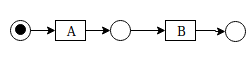
\includegraphics[width=\linewidth]{figures/introduction/PN_modelchange_a.png}
		\caption{original process model}
		\label{fig:model_a}
	\end{subfigure}
	\hfill
	\begin{subfigure}[b]{0.32\textwidth}
		\centering
		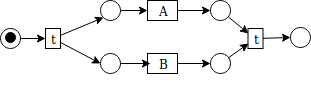
\includegraphics[width=\linewidth]{figures/introduction/PN_modelchange_b.png}
		\caption{process model \\ with high fitness}
		\label{fig:model_b}
	\end{subfigure}
	\hfill
	\begin{subfigure}[b]{0.32\textwidth}
		\centering
		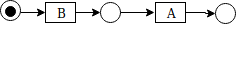
\includegraphics[width=01.0\linewidth]{figures/introduction/PN_modelchange_c.png}
		\caption{process model \\ with good KPI}
		\label{fig:model_c}
	\end{subfigure}
	
	\caption{example for model change under model repair}
	\label{fig:model_examples}
\end{figure}

However, it's obvious that $<A,B>$ often leads to bad performance and therefore should be excluded. The Figure \ref{fig:model_examples}(c) shows the expected model with incorporating the negative information. This model reinforces positive examples and avoids negative instances, which provides us a more accurate view of the business process.

The demand to repair model with incorporating negative instances appears. The concrete problem showing with demand is as follows. Given an input of one existing process model M, an event log L and KPIs, how  to improve current process enhancement techniques by incorporating negative information within process model repair, and generate a process model to enforce the positive instances while blocking the negative instance. Therefore, the repaired model provides a better way to understand and execute the real business process.


%% Problem definition

This paper tries to provide a solution for it. The reminder is organized in the following order. Section 2 recalls the basic notions on process mining and list the preliminary to solve the problem. The next section lists our methods are introduced and formal definitions are given. In Implementation Section, the details of algorithms are given. Later, we evaluate our methods with simulated data and real data respectively and list the results. Subsequently, the discussion on this paper is presented. At last section, a conclusion is drawn on the paper. 

Clearly, the use of negative information can bring significant benefits, e.g, enable a controlled generalization of a process model: the patterns to generalize should never include negative instances. 

%\end{document}